\PassOptionsToPackage{hidelinks}{hyperref}
\PassOptionsToPackage{dvipsnames,svgnames,table}{xcolor}
\documentclass[11pt,a4paper]{moderncv}
\moderncvtheme
[blue]
%[black]
%[burgundy]
%[green]
%[grey]
%[orange]
%[purple]
%[red]          
{classic}   
%{casual}  
%{classic}
%{oldstyle}
%{banking}
%{fancy}
  

\usepackage[serbian, french, english]{babel}
 \usepackage[utf8]{inputenc}

\usepackage{fontspec}
\usepackage{newunicodechar}
%\usepackage{serbian-def-cyr} % pour les lettres cyrilliques
\usepackage{mathtools,amssymb,amsthm}
\frenchsetup{StandardLayout = true}
\usepackage{enumitem}

\usepackage{pstricks}
%\usepackage{graphicx}
\usepackage[top=2cm, bottom=0.5cm, left=2cm, right=2cm]{geometry}
\usepackage{hyperref}
\hypersetup{
    colorlinks=true,
    linkcolor=blue,
    filecolor=magenta,      
    urlcolor=blue,
}

\usepackage{amsmath}
%\frenchbsetup{StandardLists=true}  % pour que l'option des listes françaises avec tiret n'apparaisse pas !!! OnionJack forever !!!



%%%%%% additional commands  %%%%%%


\newcommand{\Co}{\mathbb {C}}
\newcommand{\R}{\mathbb {R}}
\newcommand{\N}{\mathbb {N}}
\newcommand{\Q}{\mathbb {Q}}
\newcommand{\Sk}{\mathbb {S}}


\renewcommand{\Re}{\mathfrak{Re}}
%\newcommand{\Im}{\mathfrak{Im}}
 
\newcommand{\cio}{\llbracket}
\newcommand{\cif}{\rrbracket}

\newcommand{\Bc}{\mathcal{B}}
\newcommand{\Cc}{\mathcal{C}}
\newcommand{\Dc}{\mathcal{D}}
\newcommand{\Fc}{\mathcal{F}}

\newcommand{\Lc}{\mathcal{L}}

\newcommand{\Sc}{\mathcal{S}}

\newcommand{\norme}[1]{|\!| #1|\!|}


\newcommand{\Id}{\mathrm{Id}}

\newcommand{\Lop}{\mathrm{L}}
\newcommand{\ds}[1]{\underline{\underline{#1}}}
%\renewcommand{\v}[1]{\vec{#1}}


\DeclareMathOperator{\argmin}{\mathop{argmin}}
\DeclareMathOperator{\card}{\mathop{Card}}
\DeclareMathOperator{\id}{\mathop{Id}}
\DeclareMathOperator{\var}{\mathop{Var}}
\DeclareMathOperator{\vect}{\mathop{Vect}}
\DeclareMathOperator{\Lun}{\mathop{L}^1}
\DeclareMathOperator{\Ld}{L^2}
\DeclareMathOperator{\Lm}{L}
\DeclareMathOperator{\D}{d\!}
\DeclareMathOperator{\DD}{D}
\DeclareMathOperator{\esp}{E}
\DeclareMathOperator{\pr}{P}
\DeclareMathOperator{\signe}{signe}

\renewcommand{\esp}{\mathrm{\mathbf{E}}}
\newcommand{\espc}[1]{\esp\left[ #1 \right]}
\newcommand{\app}[5]{
#1  \left\{  
\begin{array}{ccl}
#2 & \longrightarrow  &#3 \\
#4 & \mapsto & #5
\end{array}
 \right.
}
 
\newcommand{\vece}[1]{\vec{#1}\;} 
 
 
%\newcommand{\defee}{\stackrel{\mbox{\begin{tiny}
% def
% \end{tiny}}}{=}}
 \newcommand{\tend}[2]{\mathop{\longrightarrow}\limits_{#1\rightarrow #2}}

\newcommand{\defe}{:=}
\newcommand{\defed}{=:}









% Largeur de la colonne pour les dates
\setlength{\hintscolumnwidth}{2.5cm}
\vspace*{-20pt}

\renewcommand*{\namefont}{\fontsize{20}{40}\mdseries\upshape}
\firstname{Ljudmila}
\familyname{PETKOVIĆ}
%\title{Postdoctorant à l'École des Mines  de Saint-Étienne}   
%\renewcommand*{\titlefont}{\fontsize{12}{40}\mdseries\upshape}  
%\title{Étudiante post-grade à l'Université de Genève}     
 
     

% \address{Korean House, International University Campus in Paris\\9G Boulevard Jourdan, apt. 716\\}{75014 Paris, France}    



%%\homepage{www.madrzejewski.com}
%\mobile{+33 (0)7 68 81 83 47}

\usepackage{academicons}
\providecommand*\orcidsocialsymbol{}\renewcommand*\orcidsocialsymbol{{\aiOrcid}~}
\social[orcid][orcid.org/0000-0003-2694-4096]{0000-0003-2694-4096}
\usepackage{graphicx}
\graphicspath{ {img/} }
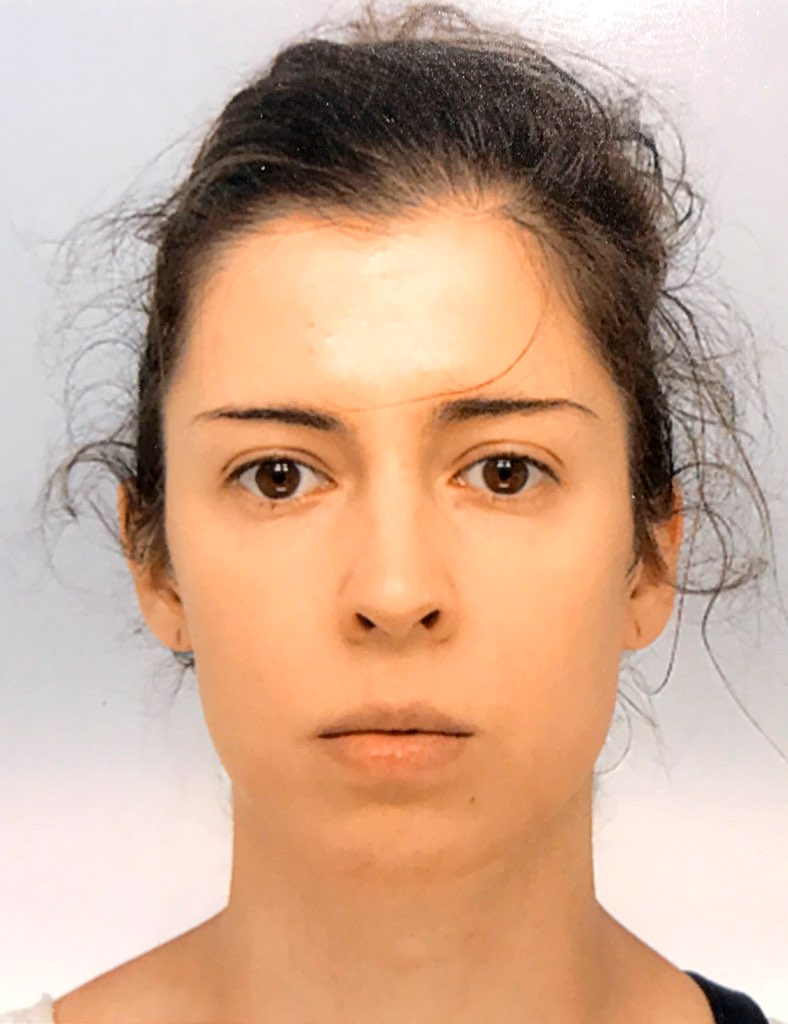
\includegraphics[width=1in, height=1.3in]{photo.jpg}


\begin{document}
\email{ljudmila.petkovic@sorbonne-universite.fr}
%\email{}
\vspace*{10pt}

\maketitle
\vspace*{-40pt}

\vspace{10pt}

\section{\textbf{Research Interests}}
My research focuses on Digital Humanities, Natural Language Processing and Deep Learning. I am particularly interested in the methods of dissemination, sharing and valorisation of heritage collections through the prism of Digital Humanities in order to track the circulation of knowledge.

\textbf{Digital Humanities}: optical character recognition (\textsc{OCR}), handwritten text recognition (\textsc{HTR}), data structuring in \textsc{XML-TEI} format, publication of queryable digital editions

\textbf{Natural Language Processing}: text mining, computational linguistics

\textbf{Deep Learning}: Transformers Models

\vspace*{4pt}
\section{\textbf{Education and Qualifications}}

%\cventry{2018 -- }{Doctorante, programme Systèmes Intelligents}{Université de Belgrade}{}{}{}{}
%
%\cventry{2017 -- }{Master en Informatique et statistiques appliquées à lalinguistique}{Université de Belgrade}{}{}{Titre du mémoire : Création et analyse d'un corpus de paroles provenant des groupes de rock yougoslaves entre les années 1950 et 2000 (soutenance prévue en mars 2019)}{}{}


\cventry{2021 -- }{PhD in Digital Humanities}{Sorbonne University, Paris (France), Faculty of Arts, Languages, Literature and Humanities, Doctoral School III \og{}French and Comparative Literature\fg{} (\textsc{ED} 019), \textsc{UMR} 8599, \textsc{CELLF} (Center for the Study of French Language and Literature), \textsc{ObTIC} (Observatory of Texts, Ideas and Corpora)}{}{}{}

\cventry{2019 -- 2024}{Certificate of specialisation in Linguistics}{University of Geneva (Switzerland), Faculty of Humanities, Department of Linguistics}{}{}{Dissertation title : Analysis of lexical fields in the heritage collection of Jean-Martin Charcot}

\cventry{2017 -- 2019}{Master in Social Sciences and Computing}{University of Belgrade (Serbia), interdisciplinary study program}{}{}{Master’s Thesis title: \textsc{Creation and Analysis of the Yugoslav Rock Song Lyrics Corpus from 1945 to 2003} [\href{https://doi.org/10.5281/zenodo.5717363}{\texttt{Zenodo}}]\\{\scriptsize\textbf{Abstract:} The thesis analyzes, from the theoretical and practical perspective, the creation and processing of corpus of rock songs’ lyrics originating from the former Yugoslavia in the period 1945-2003. The lyrics are obtained from the LyricWiki website using the Python library \texttt{lyricsmaster} in the \textit{web scraping} process. The collected texts are then merged into a single \textsc{XML} file and automatically annotated with the \texttt{yattag} Python tool. Afterwards, the data preprocessing was conducted at the formal and content level. Furthermore, the \textsc{XML} document is transformed into \textsc{XHTML} format applying \textsc{XSLT} processor, in order to generate basic corpus data. The diacritic restoration process with the ``Slovo Majstor'' application and morphological electronic dictionaries of Serbian language in the LeXimir software package, is also automated. The \textit{text mining} process encompassed retrieving socio-political and patriotic topics using \texttt{NLTK} library in Python, while romantic and other topics were visualized using the TreeCloud and WordItOut software. The similarity between authors represented in the corpus was measured using \texttt{stylo} package in the programming language \textsc{R}. Finally, an overview of the today’s most relevant programming libraries in the field of \textit{natural language processing} is provided, which, at the same time, serves as a guideline for the future work.\\ \textbf{Keywords:} corpus linguistics, Yugoslav rock and roll, web scraping, natural language processing, text mining.}
}{}{}{}

\cventry{2017 -- 2018}{Master in Language, Literature, Culture}{University of Belgrade (Serbia), Faculty of Philology}{}{}{Master’s Thesis title: \textsc{Use of the Moodle Platform in the Reformed Teaching of Neohellenistic Studies} [\href{https://doi.org/10.5281/zenodo.5717369}{\texttt{Zenodo}}]\\ {\scriptsize\textbf{Abstract:} This paper deals with the Modern Greek language and literature learning using the Moodle electronic platform within the \textit{hybrid} and \textit{online} learning model. The subject of the discussion are the main features of this teaching method, as well as the application of Moodle in working with the first-year undergraduate students of the Department of Neohelenistic Studies at the Faculty of Philology, University of Belgrade. We examine the effectiveness of the mixed-mode learning by presenting the electronic contents that are available on the online courses \textit{Contemporary Greek Language G-1} and \textit{G-2}, \textit{Greek Literature 1} and \textit{Practicum in Neohelenistics 2}. Special attention is devoted to the analysis of the course interactivity, multimediality, and flexibility. Finally, we also expose the results of the accompanying empirical research, which led to the conclusion that the implementation of Moodle in teaching significantly helps students in learning.\\
\textbf{Keywords:} hybrid learning, Moodle, modern Greek language, literature, university teaching.}
}{}{}{}
\newpage

\cventry{2013 -- 2017}{Bachelor in Modern Greek language, literature, culture}{University of Belgrade (Serbia), Faculty of Philology, Department of Neohellenic Studies}{}{}{}
  
\cventry{2009 -- 2013}{Philological High School, Belgrade (Serbia)}{French class}{}{}{}

%
\vspace*{4pt}

\section{\textbf{Work Experience}}
%\subsection{\textbf{Internship}}
%\cvitem{2018.}{Assistance in organizing the activities held by the Serbian Qigong Association.}{}{}{}{}
%\subsection{\textbf{Translation}}
\vspace*{2pt}
\cvitem{}{%
The volumes are reported in equivalent \textsc{TD} hours (\textsc{HETD}).
}{}{}{}{}
\cvitem{2024-2026}{%
%Les volumes sont renseignés en heures équivalent TD (HETD)\\
    \textsc{ATER} (Temporary Teaching and Research Associate), Sorbonne University, \textsc{UFR} Sociology and Computer Science for the Humanities, Bachelor's in Language Sciences and Master's in Language and Computing.%
    %
    \vspace{0.2cm}
    \hspace{1cm} % Adjust spacing to align the table with the ATER text
\renewcommand{\arraystretch}{1.3} % Increase row height
\hspace{1.5cm} % Adjust this value to control the right shift
\setlength{\tabcolsep}{5pt} % Adjust cell padding
\renewcommand{\arraystretch}{1.3} % Adjust row height
\hspace{1.5cm} % Shift table slightly to the right
\resizebox{0.838\textwidth}{!}{
\begin{tabular}{|p{5cm}|c|c|c|c|}
\hline
\multicolumn{1}{|c|}{\textbf{Label \textsc{ELP}}}                       & \textbf{Code \textsc{ELP}} & \textbf{Audience}       & \textbf{Year}       & \textbf{Volume}             \\ \hline
\begin{tabular}[l]{@{}l@{}}\href{https://moodle-lettres-24.sorbonne-universite.fr/course/view.php?id=3866}{Représentation et traitement}\\\href{https://moodle-lettres-25.sorbonne-universite.fr/enrol/index.php?id=4146}{des documents électroniques}\end{tabular} & \textsc{M1SOL041} & \textsc{M1}           & 2025-2026                  & \begin{tabular}[l]{@{}l@{}}\textsc{CM}: 10,5 \\ \textsc{TD} : 10,5\end{tabular} \\ \hline
\begin{tabular}[l]{@{}l@{}}\href{https://moodle-lettres-24.sorbonne-universite.fr/course/view.php?id=3866}{Introduction au traitement}\\\href{https://moodle-lettres-25.sorbonne-universite.fr/enrol/index.php?id=4146}{automatique des langues}\end{tabular} & \textsc{M2SOL035} & \textsc{M1}           & 2025-2026                  & \begin{tabular}[l]{@{}l@{}}\textsc{CM}: 16,5 \\ \textsc{TD} : 16,5\end{tabular} \\ \hline
\begin{tabular}[l]{@{}l@{}}\href{https://moodle-lettres-24.sorbonne-universite.fr/course/view.php?id=3866}{Corpus, ressources et}\\\href{https://moodle-lettres-24.sorbonne-universite.fr/course/view.php?id=3866}{linguistique outillée}\end{tabular} & \textsc{M2SOL034} & \textsc{M1}           & 2024-2025                  & \begin{tabular}[l]{@{}l@{}}\textsc{CM}: 10,5 \\ \textsc{TD} : 10,5\end{tabular} \\ \hline
\href{https://moodle-lettres-25.sorbonne-universite.fr/course/view.php?id=256}{IA hybride et machine learning}                       & \textsc{L6SOIAAU} & \textsc{L3}           & 2025-2026                 & \begin{tabular}[l]{@{}l@{}}\textsc{CM}: 15 \\ \textsc{TD} : 24\end{tabular} \\ \hline
\href{https://moodle-lettres-24.sorbonne-universite.fr/course/view.php?id=69}{Statistiques inférentielles}                       & \textsc{L6SOSTAT} & \textsc{L3}           & 2024-2025                 & \textsc{TD} : 10,5             \\ \hline
\href{https://moodle-lettres-24.sorbonne-universite.fr/course/view.php?id=68}{Mathématiques}                       & \textsc{L5SOMATH} & \textsc{L3}           & 2024-2025                  & \textsc{TD} : 9             \\ \hline
\begin{tabular}[l]{@{}l@{}}\href{https://moodle-lettres-24.sorbonne-universite.fr/course/view.php?id=483}{Recherche d'information et}\\\href{https://moodle-lettres-24.sorbonne-universite.fr/course/view.php?id=483}{site web}\end{tabular} & \textsc{L3SOWEB1} & \textsc{L2}           & 2024-2025                  & \textsc{TD} : 76\\ \hline
\begin{tabular}[l]{@{}l@{}}\href{https://moodle-lettres-24.sorbonne-universite.fr/course/view.php?id=71}{\textsc{PIX} -- Formation aux compé-}\\
\href{https://moodle-lettres-24.sorbonne-universite.fr/course/view.php?id=71}{tences numériques}\end{tabular}                                & \textsc{PIX@S2N2} & \textsc{L1} / \textsc{L2} / \textsc{L3} & 2024-2026                  & \begin{tabular}[l]{@{}l@{}}\textsc{CM}: 3 \\ \textsc{TD} : 166,5\end{tabular} \\ \hline
\href{https://moodle-lettres-24.sorbonne-universite.fr/course/view.php?id=66}{Analyse de discours avec
programmation}                       & \textsc{L2SOPROG} & \textsc{L1}           & 2024-2025                & \textsc{TD} : 2             \\ \hline
\multicolumn{5}{|c|}{\hfill\textbf{TOTAL : 381}} \\
\hline
\end{tabular}%
}
}{}{}{}{}


\cvitem{2023-2024}{\textsc{Teaching Assistant (TA)}, course ``In-depth Studies -- Digital Corpora (H5MUAB7)'', in the Master 2 Archives and the Master 2 Information and Library Sciences, (SIB), University of Angers, Angers (France), Faculty of Languages, Humanities and Social Sciences (LLSH), 3h tutorial classes, [\href{https://github.com/ljpetkovic/Formation_HTR-Transkribus_UAngers_010224/tree/master}{\texttt{link}}].}{}{}{}{}

\cvitem{2023-2024}{%
    {\textsc{Teaching Assistant (TA)}, Sorbonne Nouvelle, Paris (France), \textsc{UFR} Literature, Linguistics, Didactics (\textsc{LLD}) -- Institute of General and Applied Linguistics and Phonetics (\textsc{ILPGA}), Academic Minor \textit{Digital Humanities}}%
    \vspace{0.2cm}
    \hspace{1cm} % Adjust spacing to align the table with the ATER text
\renewcommand{\arraystretch}{1.3} % Increase row height
\hspace{1.5cm} % Adjust this value to control the right shift
\setlength{\tabcolsep}{5pt} % Adjust cell padding
\renewcommand{\arraystretch}{1.3} % Adjust row height
\hspace{1.5cm} % Shift table slightly to the right
\begin{tabular}{|p{5cm}|c|c|c|c|}
\hline
\multicolumn{1}{|c|}{\textbf{Label \textsc{ELP}}}                       & \textbf{Code \textsc{ELP}} & \textbf{Audience}       & \textbf{Year}       & \textbf{Volume}             \\ \hline
\begin{tabular}[l]{@{}l@{}}\href{https://github.com/ljpetkovic/IHN_L1HN001}{Introduction to Digital}\\\href{https://github.com/ljpetkovic/IHN_L1HN001}{Humanities}\end{tabular}                                & \textsc{L1HN001} & \textsc{L1} & 2023-2024                  & \begin{tabular}[l]{@{}l@{}}\textsc{TD} : 26\end{tabular} \\ \hline
\begin{tabular}[l]{@{}l@{}}\href{https://github.com/ljpetkovic/CNA_L2HN001}{Advanced Digital Cultures}\end{tabular} & \textsc{L2HN001} & \textsc{L1}           & 2023-2024                  & \textsc{TD} : 26            \\ \hline
\end{tabular}%
}{}{}{}{}
%\cvitem{2023-2024}{\textsc{Teaching Assistant (TA)}, course \og{}Advanced Digital Cultures\fg{}, in the Academic Minor \textit{Digital Humanities}, Sorbonne Nouvelle, Paris (France), \textsc{UFR} Literature, Linguistics, Didactics (\textsc{LLD}) -- Institute of General and Applied Linguistics and Phonetics (\textsc{ILPGA}), 26h tutorial classes, [\href{https://github.com/ljpetkovic/CNA_L2HN001}{\texttt{link}}].}{}{}{}{}

%\cvitem{2023-2024}{\textsc{Teaching Assistant (TA)}, course \og{}Introduction to Digital Humanities\fg{}, in the Academic Minor \textit{Digital Humanities}, Sorbonne Nouvelle, Paris (France), \textsc{UFR} Literature, Linguistics, Didactics (\textsc{LLD}) -- Institute of General and Applied Linguistics and Phonetics (\textsc{ILPGA}), 24h tutorial classes, [\href{https://github.com/ljpetkovic/IHN_L1HN001}{\texttt{link}}].}{}{}{}{}



\cvitem{2021 -- }{PhD in Digital Humanities, Sorbonne University, Paris (France), Faculty of Arts \& Humanities, Doctoral School III \og{}French and Comparative Literature\fg{} (\textsc{ED} 019), \textsc{UMR} 8599, \textsc{CELLF} (Center for the Study of French Language and Literature), 
\textsc{ObTIC} (Observatory of Texts, Ideas and Corpora).}{}{}{}{}

\cvitem{2021 --}{\textsc{External contributor} within the  \href{https://www.unige.ch/fapse/idea/}{\textsc{idEA}} project for the linguistic annotation task, Faculty of Psychology and Educational Sciences, University of Geneva (Switzerland), under the supervision of D\textsuperscript{r} Joanna Blochowiak.}{}{}{}{}

\cvitem{2021 -- }{Intern at the Observatory of Literary Life (laboratory of excellence \textsc{OBVIL}), as part of the \textit{Very Large Library} project (Très Grande Bibliothèque -- \href{http://obvil.lip6.fr/tgb/}{TGB}) to improve the quality of \textsc{OCR} in the \textsc{TGB} for the task of Named Entity Recognition (\textsc{NER}), Sorbonne University, Paris (France), under the supervision of Prof. D\textsuperscript{r} Glenn Roe and D\textsuperscript{r} Motasem Alrahabi.}{}{}{}{}

\cvitem{2021}{Source entry operator for the project \textsc{FNS} \href{https://www.unige.ch/visualcontagions/}{\textit{Visual Contagions}} (exhibition catalogues, \textsc{OCR-XML-TEI-CSV}) [\href{https://gitlab.unige.ch/Beatrice.Joyeux-Prunel/visual-contagions/-/tree/master/IIIFmanifests}{\texttt{GitLab}}], Faculty of Humanities, Chair of Digital Humanities, University of Geneva (Switzerland), under the supervision of Prof. D\textsuperscript{r} Béatrice Joyeux-Prunel.}{}{}{}{}

\cvitem{2020}{Scientific collaborator and research engineer within the project \textsc{FNS} \href{https://www.unige.ch/lettres/humanites-numeriques/recherche/projets-de-la-chaire/mss}{\textit{Manuscripts for Sale: Automatic Structuration and Annotation of Catalogues with Complex Layouts (Katabase)}}, Faculty of Arts and Humanities,
Institute of French Literature, University of Neuchâtel : OCRisation (in Transkribus and Kraken)/\textsc{OCR} correction of the XIX\textsuperscript{th} c. manuscript sales catalogues ; semi-automatic semantic encoding and data restructuration in \textsc{TEI-XML} generated by \textsc{\textit{GROBID}}-\textit{dictionaries} for filling in the dedicated database, under the supervision of D\textsuperscript{r} Simon Gabay.}{}{}{}{}

\cvitem{2021}{Peer reviewer of the article Rozovskaya, A. (2021). ``Spelling Correction for Russian: A Comparative Study of Datasets and Methods''. \textit{Proceedings of the International Conference on Recent Advances in Natural Language Processing (\textsc{RANLP} 2021)} [\href{http://ranlp.org/ranlp2021/proceedings-20Sep.pdf}{\texttt{link}}] and [\href{https://ranlp.org/ranlp2021/pc.php}{\texttt{link}}].}{}{}{}{}

\cvitem{2019}{Peer reviewer of the article Zosa, E., \& Granroth-Wilding, M. (2019). ``Multilingual dynamic topic model''. \textit{Proceedings of the International Conference on Recent Advances in Natural Language Processing (\textsc{RANLP} 2019)} [\href{http://lml.bas.bg/ranlp2019/proceedings-ranlp-2019.pdf}{\texttt{link}}] and [\href{http://lml.bas.bg/ranlp2019/pc.php}{\texttt{link}}].}{}{}{}{}


\cvitem{2016 --}{English/Serbian/Modern Greek translations of financial contracts, Faculty of Philology, Department of Neohellenic Studies, University of Belgrade (Serbia), coordinator: D\textsuperscript{r} Anka Rađenović.}{}{}{}{}

\cvitem{2017 -- 2018}{Participation in the Portuguese-Serbian translation project of Portuguese-speaking literary works, Faculty of Philology, Instituto Camões, University of Belgrade (Serbia), coordinator: D\textsuperscript{r} Anamarija Marinović.}{}{}{}{}

%\begin{itemize}%
%\setlength\itemsep{8pt}
%\setlength{\itemindent}{1,2in}
%\item English-Greek : 87 pages;
%
%\item English-Serbian : 51 pages;
%
%\item Serbian-Greek : 46 pages. 
%
%\end{itemize}

\vspace*{2pt}

%\subsection{\textbf{Teaching}}
\cvitem{2015 -- 2016}{Private lessons in Modern Greek language for high school students.}{}{}{}{}

\cvitem{2015 -- 2016}{Student project in lexicography -- creation of the Greek-Serbian dictionary for the students of the Department of Neohellenic Studies, Faculty of Philology, University of Belgrade (Serbia), coordinator: D\textsuperscript{r} Vojkan Stojičić.}{}{}{}{}

\newpage
% \vspace*{4pt}
\section{\textbf{List of Publications}}

\vspace*{4pt}

\subsection{\textbf{Peer-reviewed Journals}}

\cvitem{2025}{\underline{Petkovic, Lj.}, Koudoro-Parfait, C., Desmarest, M.-S. \& Lejeune, G. (2025).  Bruit de fond ou valeur ajoutée ? Gérer le bruit lors des traitements informatiques des corpus linguistiques. \textit{Revue Corpus 26 – 2025}. \textsc{DOI} : \href{https://doi.org/10.4000/1364s}{\texttt{https://doi.org/10.4000/1364s}}}

\cvitem{2024}{Koudoro-Parfait, C., \underline{Petkovic, Lj.}, \& Roe, G. (2024). Analyse multilingue de l'impact de la correction automatique de la ROC sur la reconnaissance d'entités nommées spatiales dans des corpus littéraires. \textit{Revue TAL : Robustesse et limites des modèles de traitement automatique des langues, 64}(2). \url{https://www.atala.org/sites/default/files/TAL_64_2_2.pdf}}

\cvitem{2022}{\underline{Petkovic, Lj.}, Alrahabi, M. \& Roe, G. (2022). Impact de la correction automatique de l’OCR/HTR sur la tâche de reconnaissance d’entités nommées dans un corpus bruité. \textit{Journal of Information Sciences 21}(2), pp. 1-18. \url{https://doi.org/10.34874/IMIST.PRSM/jis-v21i2.36599}.
% Actes de la journée d’étude sur la robustesse des systemes de TAL, 22}. 
% [\href{http://caio-corro.fr/pdf/robustal2022.pdf\#page=22}{\texttt{link}}]
{}{}{}{}}

\cvitem{2019}{\underline{Petković, Lj.} (2019). Creation and Analysis of the Yugoslav Rock Song Lyrics Corpus from 1967 to 2003. \textit{Infotheca -- Journal for Digital Humanities}, \textit{19}(1), pp. 5-29. \href{https://hal.archives-ouvertes.fr/hal-03091121}{\texttt{<hal-03091121>}}}{}{}{}{}

\cvitem{2018}{\underline{Petković, Lj.} (2018). Upotreba onlajn platforme Mudl (Moodle) u reformisanoj nastavi Katedre za neohelenske studije Filološkog fakulteta Univerziteta u Beogradu (Use of the Online Platform Moodle in the Reformed Teaching within the Department of Neohellenic Studies at the Faculty of Philology, University of Belgrade). \textit{Metodički vidici}, \textit{9}(9), pp. 179-200. \href{https://hal.archives-ouvertes.fr/hal-03091176}{\texttt{<hal-03091176>}}}{}{}{}{}

\vspace*{4pt}

\subsection{\textbf{Peer-reviewed Colloquia}}

\cvitem{2023}{\underline{Petkovic, Lj.}, Alrahabi, M., \& Roe, G. (2023). Circulation du discours médical de Jean-Martin Charcot : premières observations. \textit{Humanistica 2023}, Humanistica, June 2023, Geneva, Switzerland \href{https://hal.science/HUMANISTICA-2023/hal-04107099v1}{\texttt{<hal-04107099>}}.}

\cvitem{2020}{Gabay, S., \underline{Petkovic, Lj.}, Bartz, A., Levenson, M. G., \& du Noyer, L. R. (2020). Katabase: À la recherche des manuscrits vendus. \textit{Humanistica 2021}, Humanistica, May 2021, Rennes, France. \href{https://hal.archives-ouvertes.fr/hal-03066108}{\texttt{<hal-03066108>}}}{}{}{}{}

\vspace*{4pt}
\subsection{\textbf{Peer-reviewed Study Days}}

\cvitem{2024}{\underline{Petkovic, Lj.}, Koudoro-Parfait, C., \& Lejeune, G. (2024). \href{https://drive.google.com/file/d/1-71lg1eCm1McSfJ4VJHTWpPgmao_uYnC/view?usp=sharing}{Mes données ou tes méthodes ? Comment trancher la responsabilité côté \textsc{TAL} ou côté \textsc{HN} quand les résultats ne sont pas au rendez-vous ?}. Poster presented at the CNRS GdR TAL study day \og{}Natural Language Processing and Digital Humanities\fg{}, 7\textsuperscript{th} November 2024, University of La Rochelle.{}{}{}{}{}}

\cvitem{2022}{\underline{Petkovic, Lj.}, Alrahabi, M., \& Roe, G. (2022). Impact de la correction automatique de l’\textsc{OCR/HTR} sur la tâche de reconnaissance d’entités nommées dans un corpus bruité. \textit{Actes de la journée d’étude sur la robustesse des systemes de TAL}, p. 22. \textsc{HAL} : \href{http://caio-corro.fr/pdf/robustal2022.pdf\#page=22}{\texttt{<hal-03853541v1>}}}{}{}{}{}
% Actes de la journée d’étude sur la robustesse des systemes de TAL, 22}. 
% [\href{http://caio-corro.fr/pdf/robustal2022.pdf\#page=22}{\texttt{lien}}]

\vspace*{4pt}
\subsection{\textbf{Peer-reviewed Congresses}}

\cvitem{2023}{Alrahabi, M., Cordova, J., Fedchenko, V., \underline{Petkovic, Lj.}, \& Roe, G. (2023). Pandore: a toolbox for digital humanities text-based workflows [résumé]. \textit{Digital Humanities 2023: Book of Abstracts}, Digital Humanities 2023. Collaboration as Opportunity. (DH2023), Graz, Austria \texttt{[\href{https://doi.org/10.5281/zenodo.8107733}{\texttt{doi}}\texttt{]}}.}


\cvitem{2018}{Stojičić, V., \& \underline{Petković, Lj.} (2018). Od oglasa do platforme Moodle -- primer dobre prakse u nastavi modernog grčkog kao stranog (From an Advertisement to the Moodle Platform -- an Example of Good Practice in Teaching Modern Greek as a Foreign Language): Paper presented at the 6\textsuperscript{th} International Congress \og{}Primenjena lingvistika danas -- jezik, književnost i interdisciplinarnost\fg{} (\og{}Applied Linguistics Today 6 -- Language, Literature and Interdisciplinarity\fg{}) Faculty of Philology, University of Belgrade, Serbia, 12–13.10.2018. [\href{https://drive.google.com/file/d/1rzU5Gk8ba-nhAWup5Z5jAjHeKdHT3TKA/view?usp=sharing}{abstract}]}{}{}{}{}

\vspace*{4pt}
\subsection{\textbf{Peer-reviewed Conferences}}

\cvitem{2022}{Cordova, J. M., Dupont, Y., \underline{Petkovic, Lj.}, Gawley, J., Alrahabi, M. \& Roe, G. (2022). Toolbox : une chaîne de traitement de corpus pour les humanités numériques. \textit{Traitement Automatique des Langues Naturelles}, July 2022, Avignon, France. pp. 11-13. \href{https://hal.archives-ouvertes.fr/hal-03701464}{\texttt{<hal-03701464>}}}{}{}{}{}

\cvitem{2020}{Gabay, S., du Noyer, L. R., Levenson, M. G., \underline{Petkovic, Lj.} \& Bartz, A. (2020), Quantifying the Unknown: How many manuscripts of the marquise de Sévigné still exist?. In \textit{Digital Humanities} \textsc{\textit{DH2020}, ADHO}, July 2020, Ottawa, Canada. \href{https://hal.archives-ouvertes.fr/hal-02898929}{\texttt{<hal-02898929>}}}{}{}{}{}



%\cvitem{2020}{Clérice, Th., Gabay, S., \underline{Petkovic, Lj.}, Corbières, C. (2020). Detecting bold and italic in 19\textsuperscript{th} c. prints, à soumettre.}}{}{}{}{}










\cvitem{2018}{\underline{Petković, Lj.} (2018). Implementacija tehnika analize teksta u programskom jeziku Python pomoću \texttt{NLTK}-a (Implementation of text mining techniques using \texttt{NLTK} in Python programming language). In \textit{2018 26\textsuperscript{th} Telecommunications Forum (TELFOR 2018)}, pp. 975-979. \textsc{IEEE}. \href{https://hal.archives-ouvertes.fr/hal-03091167}{\texttt{<hal-03091167>}}}{}{}{}{}{}

\vspace*{4pt}
\subsection{\textbf{Peer-reviewed Workshops}}
%  (Implementation of text mining techniques using NLTK in Python programming language). 

\cvitem{2021}{Scius Bertrand, A., Gabay, S., \underline{Petkovic, Lj.}, Janes, J., Corbières, C., \& Clérice, T. (2021). The BIR database – Identifying typographic emphasis in list-like historical documents. \textit{HIP@ICDAR21 — The 6\textsuperscript{th} International Workshop on Historical Document Imaging and Processing}, September 2021, Lausanne, Switzerland. \href{https://hal.archives-ouvertes.fr/hal-03355683}{\texttt{<hal-03355683>}}}{}{}{}{}
%\cventry{Nov. 2018.}{Petković, Lj. (2018). Implementacija tehnika analize teksta u programskom jeziku Python pomoću NLTK-a (Implementation of text mining techniques using NLTK in Python programming language). In 26th Tеlеcommunicаtions Forum (TELFOR) (pp. 975-979). IEEE.}{}{}{}{}

\vspace*{4pt}
%\subsection{\textbf{Peer-reviewed Posters}}
%\cvitem{2024}{\underline{Petkovic, Lj.}, Koudoro-Parfait, C., \& Lejeune, G. (2024). \href{https://drive.google.com/file/d/1-71lg1eCm1McSfJ4VJHTWpPgmao_uYnC/view?usp=sharing}{Mes données ou tes méthodes ? Comment trancher la responsabilité côté \textsc{TAL} ou côté \textsc{HN} quand les résultats ne sont pas au rendez-vous ?}. Journée d'étude du \textsc{GdR TAL CNRS} \og{}Traitement Automatique des Langues et les Humanités Numériques\fg{}, le 7 novembre 2024, université La Rochelle.{}{}{}{}{}}
%\cvitem{2018.}{Стојичић, В., \textbf{Петковић, Љ.} (2018). Од огласа до платформе MOODLE -- пример добре праксе у настави модерног грчког као страног језика (D'une publicité à la plateforme Moodle -- un exemple de bonne pratique dans l'enseignement du grec moderne comme langue étrangère): Papier présenté au 6\ieme congrès international Примењена лингвистика данас -- језик, књижевност и интердисциплинарност” (La linguistique appliquée aujourd'hui -- langue, littérature et interdisciplinarité) (Belgrade, 12–13.10.2018).}{}{}{}{}




%\section{\textbf{Languages}}
%\cvitem{Modern Greek}{Advanced}{}
%\cvitem{English}{Advanced}{}{}
%\cvitem{French}{Advanced}{}
%\cvitem{Portuguese}{Intermediate}{}
%\cvitem{Latin, Greek}{Reading, writing}{}

\vspace*{4pt}
\section{\textbf{Talks}}
\subsection{\textbf{Conferences}}


\cvitem{2025}{\href{https://www.fabula.org/actualites/122618/le-texte-de-l-autre-dialogue-interdisciplinaire-autour-de-l-intertextualite-et-du-discours-rapporte.html}{\textsc{The Text of the Other. Interdisciplinary Dialogue on Intertextuality and Reported Speech}} -- \href{https://github.com/ljpetkovic/Colloque_Intertextualite_030725/blob/main/0_main.pdf}{\color{purple!60!black}{\og{}Analysis of the Scientific Impact of Jean-Martin Charcot on French Medical Literature from the 19\textsuperscript{th} to the 20\textsuperscript{th} century\fg{}}}, organised by the Center for Interlingual Research on Meaning in Context (\textsc{CRISCO}). Sorbonne Nouvelle, Maison de la Recherche | École des Chartes, 1-3 July 2025, Paris (France).}{}{}{}{}

\cvitem{2023}{\textbf{\textsc{\textsc{Humanistica 2023}}} -- 4\textsuperscript{th} edition of the Humanistica conference. 23\textsuperscript{th}-28\textsuperscript{th} June 2023, Geneva (Switzerland) [\href{https://humanistica2023.sciencesconf.org/program/details}{\texttt{link}}].}{}{}{}{}

\cvitem{2022}{\textbf{\textsc{\textsc{CIHN'22}}} -- International Conference \textsc{CIHN'22} \og{}Digital humanities at the centre of the management of cultural heritage, data and information. Methods, devices and perspectives\fg{}. 22-23 November 2022, Rabat (Morocco) [\href{https://cihn22.sciencesconf.org/data/pages/CIHN22_Programme_7.pdf}{\texttt{link}}].}{}{}{}{}
\cvitem{2022}{\textbf{\textsc{UNIGE Data Science Day}} -- \og{}Promises of Artificial Intelligence\fg{}, 15\textsuperscript{th} September 2022, Geneva (Switzerland) [\href{https://datascience.unige.ch/recherche/uniges-data-science-days}{\texttt{link}}].}{}{}{}{}


\cvitem{2022}{\textsc{\textbf{TALN-RÉCITAL}} -- \og{}Towards an inclusive \textsc{NLP}\fg{}, 27\textsuperscript{th} June -- 1\textsuperscript{st} July 2022, Avignon (France) [\href{https://taln2022.univ-avignon.fr/programme.php#P1}{\texttt{link}}].}{}{}{}{}

\cvitem{2021}{\textbf{Humanistica 2021}, Francophone Association of Digital Humanities, 10\textsuperscript{th}-12\textsuperscript{th} May 2021, Rennes (France) [\href{https://humanistica2021.sciencesconf.org/program/details}{\texttt{link}}].}{}{}{}{}

\cvitem{2020}{\textbf{\textsc{DH2020}} -- Digital Humanities \textsc{DH2020}, \og{}carrefours/intersections\fg{}, ADHO, 22\textsuperscript{th}-24\textsuperscript{th} July 2020, Ottawa (Canada) [\href{https://dh2020.adho.org/wp-content/uploads/2020/07/267_QuantifyingtheUnknownHowManyManuscriptsofSvignStillExist.html}{\texttt{link}}].}{}{}{}{}

\cvitem{2018}{\textbf{\textsc{TELFOR}} -- 26\textsuperscript{th} Telecommunications Forum, Centre Sava, Belgrade (Serbia), 26\textsuperscript{th}-27\textsuperscript{th} November 2018 [\href{http://2018.telfor.rs/files/Program\%20TELFOR\%202018.pdf}{\texttt{link}}].}{}{}{}{}

\vspace{0.2cm}
\subsection{\textbf{Study Days}}

\cvitem{2025}{\href{https://ihn.sorbonne-universite.fr/journee-detude-humanites-numeriques-et-intelligence-artificielle-interactions/altercations}{\textsc{Study Day: Digital Humanities and Artificial Intelligence: Interactions / Altercations}} -- poster session \href{https://drive.google.com/file/d/131p4fmHj5knRiVVIXKp5onFXPFkyGzTd/view}{\color{purple!60!black}{\og{}Analysis of Jean-Martin Charcot's Influence through Medical Terminology Extraction: a \textit{PatternRank} Approach\fg{}}}. Study day launching the Digital Humanities Initiative of Sorbonne University. Maison de la recherche, Paris (France), 7\textsuperscript{th} November 2025.}{}{}{}{}


\cvitem{2025}{\href{https://calendar.google.com/calendar/u/0/r/day/2025/6/17}{\textsc{Study Day of the \textsc{ARIANE} Consortium (\textsc{WG4})}} \og{}AI-Assisted Literary Analysis\fg{} -- \href{}{\color{purple!60!black}{\og{}...\fg{}}}, organised by the \href{https://cst-ariane.huma-num.fr/\#month}{\textsc{ARIANE} Consortium}. \textsc{SCAI}, Paris (France), 17 June 2025.}{}{}{}{}

\cvitem{2024}{\href{https://afia.asso.fr/les-journees-communes/humanite-numerique-et-ia/}{\textsc{Artificial Intelligence and Digital Humanities}} -- \href{https://github.com/ljpetkovic/JE_IA_HN_030524_BnF/blob/main/latex/0_main.pdf}{\color{purple!60!black}{\og{}Measuring Charcot’s Influence on his Contemporaries Using Keyphrase Extraction\fg{}}}. Study day organized under the aegis of the French Association for Artificial Intelligence (\textsc{AFIA}), and the \textsc{RG CNRS MADICS} and \textsc{MAGIS}, National Library of France, Paris (France), 3\textsuperscript{rd} May 2024.}{}{}{}{}

\cvitem{2023}{\textbf{Background noise or added value? Managing noise during computer processing of linguistic corpora} --
co-organised by the University of Grenoble Alpes and Roma La Sapienza, House of Languages and Cultures, University Grenoble Alpes, Grenoble (France), 28\textsuperscript{th} April 2023 [\href{https://drive.google.com/file/d/1rna0SEBG0DRTy6IVAFl3WeXtpfbRITCC/view?usp=sharing}{\texttt{link}}].}{}{}{}{}

\cvitem{2023}{\textbf{Digital Humanities Study Day at Sorbonne University} -- 1\textsuperscript{st} study day on Digital Humanities, Maison de la recherche, Paris (France), 18\textsuperscript{th} January 2023 [\href{https://obtic.sorbonne-universite.fr/actualite/journee-humanites-numeriques-sorbonne-universite/}{\texttt{link}}].}{}{}{}{}

\cvitem{2022}{\textbf{Robus\textsc{TAL}22} -- 1\textsuperscript{st} study day on the robustness of the \textsc{NLP} systems, Maison de la recherche, Paris (France), 25\textsuperscript{th} November 2022 [\href{https://www.atala.org/sites/default/files/robustal2022.pdf}{\texttt{link}}].}{}{}{}{}

\vspace{0.2cm}
\subsection{\textbf{Congresses}}

	\cvitem{2023}{\textbf{DH2023} :
	International Conference “DH2023 -- Collaboration as Opportunity”, University of Graz | Messe Congress Graz, Graz (Austria), 10\textsuperscript{th}–14\textsuperscript{th} July 2023 [\href{https://dh2023.adho.org/}{\texttt{link}}].}{}{}{}{}
    
	\cvitem{2018}{\textbf{ALT 6}: 
	6\textsuperscript{th} International Congress “Primenjena lingvistika danas -- jezik, književnost i interdisciplinarnost” (``Applied Linguistics Today 6
– Language, Literature and Interdisciplinarity''), Faculty of Philology, Belgrade (Serbia), 12\textsuperscript{th}–13\textsuperscript{th} October 2018 [\href{http://www.fil.bg.ac.rs/wp-content/uploads/skupovi/alas-6/ALT6_program.pdf}{\texttt{link}}].}{}{}{}{}
\vspace{0.2cm}

\subsection{\textbf{Seminars}}

\cvitem{2026}{\textbf{\textsc{Seminar of the \og{}Linguistic Variation and Computational Linguistics\fg{} team}}, organised by D\textsuperscript{r} Gaël Lejeune, \href{https://drive.google.com/file/d/1PfAUj9CQWoBNw81cNqfar2XIUst8bkIT/view?usp=sharing}{\color{purple!60!black}{\og{}Tracing the circulation of concepts in noisy heritage corpora: contributions and limits of automatic tools using the Jean-Martin Charcot collection\fg{}}}. 11\textsuperscript{th} June 2026, Maison de la Recherche, Paris (France).}{}{}{}{}

\cvitem{2025}{\textbf{\textsc{ObTIC Team Doctoral Seminar}}, \textsc{SCAI}, Paris (France). Seminar organised by Prof. D\textsuperscript{r} Glenn Roe and D\textsuperscript{r} Motasem Alrahabi.
\begin{itemize}
    \item \href{https://github.com/ljpetkovic/Seminaire_doctoral_ObTIC_060225/blob/main/0_main.pdf}{\color{purple!60!black}{\og{}Measuring the Impact of Jean-Martin Charcot \textit{via} the Extraction
of Medical Terms: Which Approach to Adopt?\fg{}}}, 6\textsuperscript{th} February 2025.
\item \href{https://github.com/ljpetkovic/Seminaire_doctoral_ObTIC_130325/blob/main/0_main.pdf}{\color{purple!60!black}{\og{}Comparison of Keyphrase Extraction Approaches\fg{}}}, 13\textsuperscript{th} March 2025.
\item \href{https://github.com/ljpetkovic/Seminaire_doc_ObTIC_15-04-25/blob/main/0_main.pdf}{\color{purple!60!black}{\og{}Keyphrase Extraction from the Charcot Corpus: Quantitative and Qualitative Evaluation\fg{}}}, 15\textsuperscript{th} April 2025.
\end{itemize}
{}{}{}{}}

\cvitem{2024}{\textbf{\href{http://stih-sorbonne-universite.fr/dokuwiki/doku.php?id=seminaire\_lc}{Seminar of the \og{}Computational Linguistics -- Speed Dating\fg{} team}}, organised by D\textsuperscript{r} Gaël Lejeune, \href{https://github.com/ljpetkovic/SemVarLing_120924/blob/main/0_main.pdf}{\color{purple!60!black}{\og{}Origins and Progress of the Project Charcot\fg{}}}. 12\textsuperscript{th} September 2024, Maison de la Recherche, Paris (France).}{}{}{}{}


\cvitem{2024}{\href{https://docs.google.com/presentation/d/1GkTQaURAi3nYcn6obUXuGW4Uwqm9S2UNXxhk16mBXHA/edit?usp=sharing}{\textbf{PhD Seminar/Workshop on \textsc{HTR} and \textsc{eScriptorium}}}, organised by Centre Roland Mousnier of the Faculty of Arts, Languages, Literature and Humanities, Sorbonne University, Feedback Session, 26\textsuperscript{th} April 2024, Centre Roland Mousnier (France).}{}{}{}{}

\cvitem{2024}{\href{https://ceres.sorbonne-universite.fr/\%C3\%A9v\%C3\%A9nements/}{\textsc{PhD Seminar of the service unit Center for Experimentation in Digital Methods for Research in the Humanities and Social Sciences (\textsc{CERES}), \og{}Approaches to Digital Methods\fg{}}} -- {\href{https://github.com/ljpetkovic/Seminaire_doctoral_CERES_270324/blob/main/0_main.pdf}{\color{purple!60!black}{\og{}In Charcot's Private Papers: from Experimentation to the Premises of Modern Neurology\fg{}}}}. Seminar organised by Léa Andolfi, Julien Bezançon, Clara Bordier, Thibault Grison, Rimane Karam, Adélie Laruncet and Marine Tiger, 27\textsuperscript{th} March 2024, Maison de la Recherche, Paris (France).}{}{}{}{}

\cvitem{2023}{\textbf{Seminar for Master's students, \og{}Literary Digital Humanities\fg{}}, organised by Prof. D\textsuperscript{r} Glenn Roe, \og{}Circulation of the Jean-Martin Charcot's medical discourse: first observations\fg{}, 6\textsuperscript{th} December 2023, Maison de la Recherche, Paris (France) [\href{https://drive.google.com/file/d/1MmkNtILRNaTgQqufg6elqVkWyqPaiwgu/view?usp=sharing}{\texttt{link}}].}{}{}{}{}

\cvitem{2023}{\textbf{Doctoral seminar/workshop on \textsc{OCR} and \textsc{HTR}}, organised by Centre Roland Mousnier of the Faculty of Arts, Languages, Literature and Humanities, Sorbonne University, \og{}Digitisation of documents
transcription, annotation, OCR, HTR, correction...
\fg{}, with D\textsuperscript{r} Motasem Alrahabi, 22\textsuperscript{th} November 2023, Maison de la Recherche, Paris (France) [\href{https://docs.google.com/presentation/d/1GkTQaURAi3nYcn6obUXuGW4Uwqm9S2UNXxhk16mBXHA/edit?usp=sharing}{\texttt{link}}].}{}{}{}{}

\cvitem{2023}{\textbf{Seminar of the \og{}Computational Linguistics\fg{} team}, organised by D\textsuperscript{r} Gaël Lejeune, \og{}Automatic correction of OCR interferences in the recognition of spatial named entities: real gain or loss of information?\fg{}, 13\textsuperscript{th} April 2023, Maison de la Recherche, Paris (France) [\href{http://stih-sorbonne-universite.fr/dokuwiki/doku.php?id=seminaire_lc}{\texttt{link}}].}{}{}{}{}

\cvitem{2022}{\textbf{Seminar \og{}Literary Digital Humanities\fg{}}, organised by Prof. D\textsuperscript{r} Glenn Roe, ``Impact of automatic correction of the OCR/HTR on the named entity recognition task in noisy corpora'', 16\textsuperscript{th} November 2022, Maison de la Recherche, Paris (France) [\href{https://drive.google.com/file/d/1wM6et7j3TUOxOOV0RI7QeqTBW3-CYFaK/view?usp=sharing}{\texttt{link}}].}{}{}{}{}

\cvitem{2021}{\textbf{\textsc{JeRTeh}}, \og{}Katabase : In Search of Lost Manuscripts\fg{}, organised by \textsc{JeRTeh}, Language Resources and Technologies Society in Belgrade (Društvo za Jezičke Resurse i Tehnologije, Beograd), 10\textsuperscript{th} June 2021, Belgrade (Serbia) [en ligne] [\href{http://jerteh.rs/wp-content/uploads/2021/06/Katabase_slides.pdf}{\texttt{link}}].}{}{}{}{}

\vspace{0.2cm}
\subsection{\textbf{Workshops}}

\cvitem{2024}{\href{https://docs.google.com/document/d/1eD7RD\_-WAo7yQKKerpVMhoNtux5GqfNuaYPMnDXCji8/edit}{\textsc{\textbf{Python Workshop}}} -- \href{https://github.com/ljpetkovic/Charcot_KeyBERT_Keyphrase-Vectorizers/blob/main/pres/0_main.pdf}{\color{purple!60!black}{\og{}Keyphrase Extraction from the Charcot collection\fg{}}}, organised by the team-project \textsc{ObTIC}, 30\textsuperscript{th} April 2024, DataLab, National Library of France, Paris (France).}{}{}{}{}

\cvitem{2023 --}{\href{https://scai.sorbonne-universite.fr/public/events/view/a8046651d11c55bfbcd0/11}{\textbf{\textsc{ANHIMO} Workshop}}, \href{https://drive.google.com/file/d/1M3sO1-fXc3HOJCjEWzHIcLusL4WHwT-S/view}{\color{purple!60!black}{\og{}Use of the
Automatic Text Transcription Techniques for the Analysis of Typed Maritime Documents of the XX\textsuperscript{th} c.\fg{}}}, Summer School of Numerical Analysis of the History of the Sea and Oceans (\textsc{ANHIMO 2023}), dedicated to numerical analysis of the History of the Sea and Oceans and organised by the Ocean Institute of Sorbonne University Alliance and \textbf{S}orbonne \textbf{C}entre for \textbf{A}rtificial \textbf{I}ntelligence (\textsc{SCAI}), Paris (France), 26\textsuperscript{th}-30\textsuperscript{th} June 2023.}{}{}{}{}

\cvitem{2021}{\textbf{Python Workshop}, \og{}Handling text files\fg{}, organised by the team-project \textsc{ObTIC}, 5\textsuperscript{th} December 2021, Paris (France) [\href{https://drive.google.com/file/d/1CqWYbNkowMzfmbzqX_bMRouvZFmI5YUf/view}{\texttt{link}}].}{}{}{}{}


\cvitem{2021}{\textbf{\textsc{OCR Workshop}}, \og{}Automatic correction of the \textsc{OCR} output\fg{}, organised by the team-project \textsc{ObTIC}, 25\textsuperscript{th} November 2021, Paris (France) [\href{https://drive.google.com/file/d/13I7SxMKOLu6wkUSr0sn441O51wLOL4kD/view}{\texttt{link}}].}{}{}{}{}

\cvitem{2021}{\textbf{\textsc{OCR} Workshop}, \og{}Transkribus, Kraken, eScriptorium, Tesseract\fg{}, organised by the team-project \textsc{ObTIC}, 18\textsuperscript{th} November 2021, Paris (France), with Johanna Cordova [\href{https://drive.google.com/file/d/1ytegdE6kR78R89186G9O4w2rhTH3GcLE/view}{\texttt{link}}].}{}{}{}{}

\cvitem{2021}{\textbf{\textsc{OCR} Workshop}, \og{}Presentation and use of OCR/HTR tools: Abbyy FineReader, Transkribus, Kraken and eScriptorium\fg{}, organised by team-project \textsc{ObTIC}, 28\textsuperscript{th} October 2021, Paris (France), with D\textsuperscript{r} Motasem Alrahabi [\href{https://github.com/obtic-scai/Toolbox/blob/main/OCR/partie\%201/OCR_diapos.pdf}{\texttt{link}}].}{}{}{}{}


\newpage

\section{\textbf{Co-supervision of Master's Thesis}}

\cvitem{2025}{Camille Fief \& Yeleen Canonge (\textsc{M1} -- Sorbonne University) : \og{}\href{https://github.com/YeleenC/Memoire-Master-1-REN-sur-donnees-bruitees}{\textbf{Reconnaissance d'entités nommées et entraînement de
modèle sur données bruitées}}\fg{} (\og{}Named Entity Recognition and Model Training on Noisy Data\fg{}), with
Gaël Lejeune and Caroline Koudoro-Parfait.}{}{}{}{}{}

\cvitem{2025}{Ruixing Zheng et Marina Carvalho Lopes (\textsc{M1} -- Sorbonne University) : \og{}\href{https://github.com/MarinaaLopess/MemoireM1/}{\textbf{Reconnaissance d'Entités Nommées sur un corpus de poèmes du 19\ieme{} siècle}}\fg{} (\og{}Named Entity Recognition on a Corpus of 19\textsuperscript{th} Century Poems\fg{}), with
Gaël Lejeune and Caroline Koudoro-Parfait.}{}{}{}{}{}


\vspace*{4pt}

\section{\textbf{Additional Training}}

\cvitem{2025}{\href{https://adum.fr/phd/formation/catalogue.pl?mod=3645898&parent=moduleaccept}{\textsc{[DFC] Ethics of Scientific Research}}, organised by Sorbonne University, Campus Cordeliers, Sorbonne University, Paris (France) [participation : in person] 
% [\href{https://sites.google.com/aries.iimas.unam.mx/school-digital-humanities/about?authuser=0}{\texttt{lien}}]
[\href{}{\color{purple!60!black}{\texttt{certificate of attendance}}}].}{}{}{}{}{}

\cvitem{2023}{``Summer School on Digital Humanities'', as part of the strategic alliance between National Autonomous University of Mexico (\textsc{UNAM}) and Sorbonne Center for Artificial Intelligence (\textsc{SCAI}). Applied Mathematics and Systems Research Institute (\textsc{IIMAS}), Mexico City, Mexico 
% [\href{https://sites.google.com/aries.iimas.unam.mx/school-digital-humanities/about?authuser=0}{\texttt{link}}]
[\href{https://drive.google.com/file/d/1fjKB8wao-Cxt0Jtfg9tOp82Eamn0VY8x/view?usp=sharing}{\texttt{certificate of attendance}}].}{}{}{}{}{}

\cvitem{2022}{EnExDi (\textit{Encoder, Exploiter, Diffuser}) -- \og{}Digital humanities in research projects\fg{}, intensive training school in digital humanities, The House of the Humanities and Social Sciences (\textsc{MSHS}), University of Poitiers, France [\href{https://drive.google.com/file/d/1upYpMyEPL6F0kITjNby8aU6nNMh5AtXq/view?usp=sharing}{\texttt{certificate of attendance}}].}{}{}{}{}{}

\cvitem{2022}{\og{}Introduction to Natural Language Processing\fg{}, course offered as part of the Master \og{}Digital Humanities\fg{} of the \textsc{PSL} University (Paris Sciences \& Letters) | ENC (National School of Charters) [\href{https://drive.google.com/file/d/1h_Do8DIBqKfbZst3FikrxF1w6BZl64yi/view?usp=sharing}{\texttt{certificate of attendance}}].}{}{}{}{}{}

\vspace*{4pt}
\section{\textbf{Scholarships and Awards}}

\cvitem{2023 -- }{Travel Bursary ADHO of the DH2023 Conference, Graz (Austria) [\href{https://adho.org/awards/conference-bursary-awards/}{\texttt{link}}].}{}{}{}{}{}

\cvitem{2021 -- }{Funding of the PhD contract by the French Excellence Initiative (Idex), as part of the Institutes and Initiatives Programme of The Sorbonne University Alliance (ASU) (The Heritage Observatory -- OPUS) [\href{https://institut-opus.sorbonne-universite.fr/actualites-opus/campagne-dattribution-de-contrats-doctoraux}{\texttt{link}}].}{}{}{}{}{}

\cvitem{2017 -- 2018}{Dositeja – Serbian Government scholarship (Fund for Young Talents of the Republic of Serbia) for the best Master’s students}{}{}{}{}{}

\cvitem{2016 -- 2017}{Dositeja – Serbian Government scholarship (Fund for Young Talents of the Republic of Serbia) for the best Bachelor’s students}{}{}{}{}{}

\cvitem{2016}{Dean’s Honor. Mention for Outstanding academic achievement, University of Belgrade (Serbia), Faculty of Philology}{}{}{}{}{}

\cvitem{2014 -- 2016}{Serbian Government scholarship (Ministry of Education, Science and Technological Development) for the Bachelor’s students}{}{}{}{}{}

\cvitem{2014}{Training certificate from the Center for Lifelong Learning and Training of the University of Ioannina (Center for Greek Language Education and Culture DI.K.E.P.P.E.E. \og{}Stavros Niarchos\fg{}) – IKY scholarship for the Summer School of the Greek language and culture in Ioannina (Greece)}{}{}{}{}{}


%
%\section{\textbf{Technical skills}}
%
%%\subsection{\textbf{Informatics}}
%\cvitem{MS Office}{Word, Excel, Access, PowerPoint.}{}
%\cvitem{Programming}{Python, HTML, CSS, XML, SQL and  \LaTeX.}{}



\vspace*{4pt}
\section{\textbf{Skills}}

\subsection{\textbf{Informatics}}
\cvitem{\textsc{MS} Office}{Word, Excel, Access, PowerPoint}{}
\cvitem{\textsc{OS}}{Windows, mac\textsc{OS}, Linux}{}

\subsection{\small\textbf{Languages}}
\cvitem{Script}{Python (\texttt{os, re, numpy, matplotlib, scipy, pandas, scikit-learn, nltk, tensorflow, pytorch, gensim, requests, spacy})$\dots$, \textsc{R} (\texttt{stylo, ggplot2, knitr}), Bash, Perl}{}
\cvitem{Development}{\textsc{HTML/CSS}}{} % JavaScript}{}
\cvitem{\small Databases}{\textsc{SQL}}{}
\cvitem{Markup}{\textsc{XML}, \LaTeX, Markdown}{}
\cvitem{\small Stylesheets}{\textsc{XSLT}}{}

\subsection{\small\textbf{Version Control}}
\cvitem{}{Git}{}


\subsection{\small\textbf{Other Softwares}}
\cvitem{}{Transkribus, Kraken, eScriptorium, \textsc{TXM}, \textsc{GROBID}-dictionaries, Gephi, Docker, Oxygen \textsc{XML} Editor, Anaconda, Visual Studio Code, RenderX \textsc{XEP} Engine, \textsc{DARIAH-DE} Topics Explorer, \textsc{SPSS}, \textsc{SQL} Server Management Studio, Azure Data Studio, Unitex, PyCharm, TreeCloud, Zotero, PIX, Overleaf, Texmaker, TeXstudio}{}

\subsection{\small\textbf{Familiar with}} 
\cvitem{}{\textsc{DTS, IIIF}, \textsc{SPARQL}, Flask, Protégé, \textsc{MATLAB},  Isabelle}



\subsection{\small\textbf{Audiovisual Arts}} 
\cvitem{}{Final Cut Pro X, Sony Vegas, \textsc{FL} Studio, \textsc{MAGIX}, Audacity, Virtual \textsc{DJ}}

\vspace*{4pt}
\subsection{\textbf{Languages}}
\cvlanguage{Serbian}{Native}{}
\cvlanguage{Français}{Fluent}{}
\cvlanguage{Anglais}{Fluent}{}
\cvlanguage{Grec moderne}{Fluent}{}
\cvlanguage{Portugais}{Intermediate}{}
\cvlanguage{Coréen}{Beginner}{}
\cvlanguage{Latin}{Reading, writing}{}
\cvlanguage{Grec ancien}{Reading, writing}{}



% \section{\textbf{Scientific interests}}
% \subsection{\textbf{Digital Humanities}}
%\cventry{}{}
%\begin{itemize}%
%\setlength\itemsep{8pt}
%\setlength{\itemindent}{1,2in}
%\item General and Computational Linguistics
%\item Natural Language Processing, Text Mining
%\item Data Science
%\item Programming languages 
%\end{itemize}{}{}{}{}{}{}
% \begin{itemize}[leftmargin=+1.2in]
% \item Artificial Intelligence
% \begin{itemize}
% \vspace{-0.2cm}\item Natural Language Processing (Text Mining)
% \vspace{-0.1cm}\item Machine / Deep Learning
% \vspace{-0.1cm}\item Optical Character Recognition (\textsc{OCR})/Handwritten Text Recognition (\textsc{HTR}), automatic correction of the \textsc{OCR/HTR} output
% \end{itemize} 

% \vspace{-0.2cm}\item Statistical methods in Social Sciences 
% \vspace{-0.2cm}\item Data Visualisation (stylometry, cartography, network analysis)
% \end{itemize}

% \vspace*{4pt}
% \subsection{\textbf{Linguistics}}
% \begin{itemize}[leftmargin=+1.2in]
% \item Computational
% \vspace{-0.2cm}\item Corpus Linguistics
% \vspace{-0.2cm}\item Comparative (historical)
% %\vspace{-0.2cm}\item Cognitive 
% %\vspace{-0.2cm}\item Ancient and modern 
% \end{itemize}

% \subsection{\textbf{Philology}}
% \begin{itemize}[leftmargin=+1.2in]
% \item Comparative (historical)
% \vspace{-0.2cm}\item Classical and modern
% \end{itemize}

\vspace*{4pt}
\section{\textbf{Sports Experience}}

\cvitem{2024 --}{taekwondo -- violet belt (XX \textit{keup}), club SP Training, Bourg-la-Reine (France).} 


\cvitem{2021 -- 2023}{taekwondo -- blue belt-two red stripes (4\textsuperscript{th} \textit{keup}), club Paris Taekwondo Elite, Paris (France).}
\cvitem{2019 -- 2021}{taekwondo -- green belt-blue stripe (5\textsuperscript{th} \textit{keup}), club Il Gi Dojang, Geneva (Switzerland).}
\cvitem{2015 -- 2019}{taiji quan -- club \og{}Peng\fg{}, Belgrade (Serbia).}
\cvitem{2015 -- 2019}{qigong -- certificate of participation in modules I and II for the instructor of qigong, Serbian qigong federation, Belgrade (Serbia).}

\vspace*{4pt}
\section{\textbf{Other Interests}}
\cvitem{2018 -- 2019}{Member of the Society for Language Resources and Technologies in Belgrade (Serbia) \textsc{JeRTeh} (Društvo za Jezičke Resurse i Tehnologije, Beograd [\href{http://jerteh.rs}{\texttt{link}}])}  
\begin{itemize}
\setlength\itemsep{2pt}
\setlength{\itemindent}{1,2in}
\item Audiovisual arts
\vspace{-0.1cm}\item Eastern Asian languages and cultures (Chinese, Japanese, Korean)
\end{itemize}



\end{document}
